\section{Methodology}\label{sec:methodology}
In order to answer the research questions as posed in section \ref{sec:introduction}, two test environments will be used. The first environment will be used to perform an automated in-place migration of a node between Puppet and Ansible. The second environment contains a single node running \texttt{mgmt}. This environment will be used to perform a proof of concept implementation of a web server in \texttt{mgmt}. Both environments will be discussed in chronological order below. 

\subsection{Node migration}
During this report we repeatedly write about a merge scenario. This report is written assuming that ultimately one CMS is chosen to manage the whole IT infrastructure. As such we merge two systems by migrating them from a legacy CMS to a new one. In this (primary) test scenario a server running an Apache web server will be migrated between Puppet and Ansible. Apache was chosen for the fact that there is a lot of documentation available on this specific software package. The environment has been set up in VMware Workstation and contains a Puppet master, an Ansible server, and two Ubuntu servers (14.04 LTS) in the role of a client. This is also illustrated in figure \ref{fig:situation1} and figure \ref{fig:situation2}. One of the client servers is managed by Puppet and the second is managed by Ansible. All of these systems have been placed in the same subnet, omitting the need for specific routing or firewall configurations. 

This test is performed to see if the migration idea is feasible and to identify prerequisites migration teams have to deal with before migrating. When a company is running just two servers of a single type it might not be that useful. A new machine could be spun up easily and configured by the new configuration management system. For a small company this might be the most effective method. But in a large server farm running hundreds of web servers spinning up one server to replace one production server takes to much time. Migrating all webservers within seconds without the service going down is the best case scenario. First a methodology for a node migration from Puppet to Ansible is discussed. Subsequently the reverse scenario is drawn up. 

\subsubsection{Migrating from Puppet to Ansible}\label{subsec:Puppettoansible}
This scenario describes a migration form Puppet to Ansible in which Company A uses Puppet natively and Company B uses Ansible by default. In a situation where Ansible is decided upon as the ultimate CMS, all clients under control of the Puppet Master need to be migrated to the Ansible environment. Prior to migrating the clients, some prerequisites need to be fulfilled in order to prevent loss of functionality. As explained in section \ref{sec:background}, Puppet and Ansible are different in the way they send commands to the clients. Where Puppet is a pull based management system, Ansible is a push based system. In short: Puppet clients check in to the Puppet master to see if there are any new jobs to execute and to see if the configuration is still in the correct state. Ansible connects to the clients over a SSH session to deliver new jobs to execute. In figure \ref{fig:situation1} "Client1" is under control of the Puppet Master. In a real world scenario, this could be expanded to a farm of (web)servers. The Ansible server needs to be able to connect to the webservers in this client group over TCP port 22. All Puppet modules to be migrated need to be reproduced within Ansible as playbooks. This way the exact functionality of the environment prior to the migration can be guaranteed when the environment comes under control of a new CMS.

\begin{figure}[!ht]
        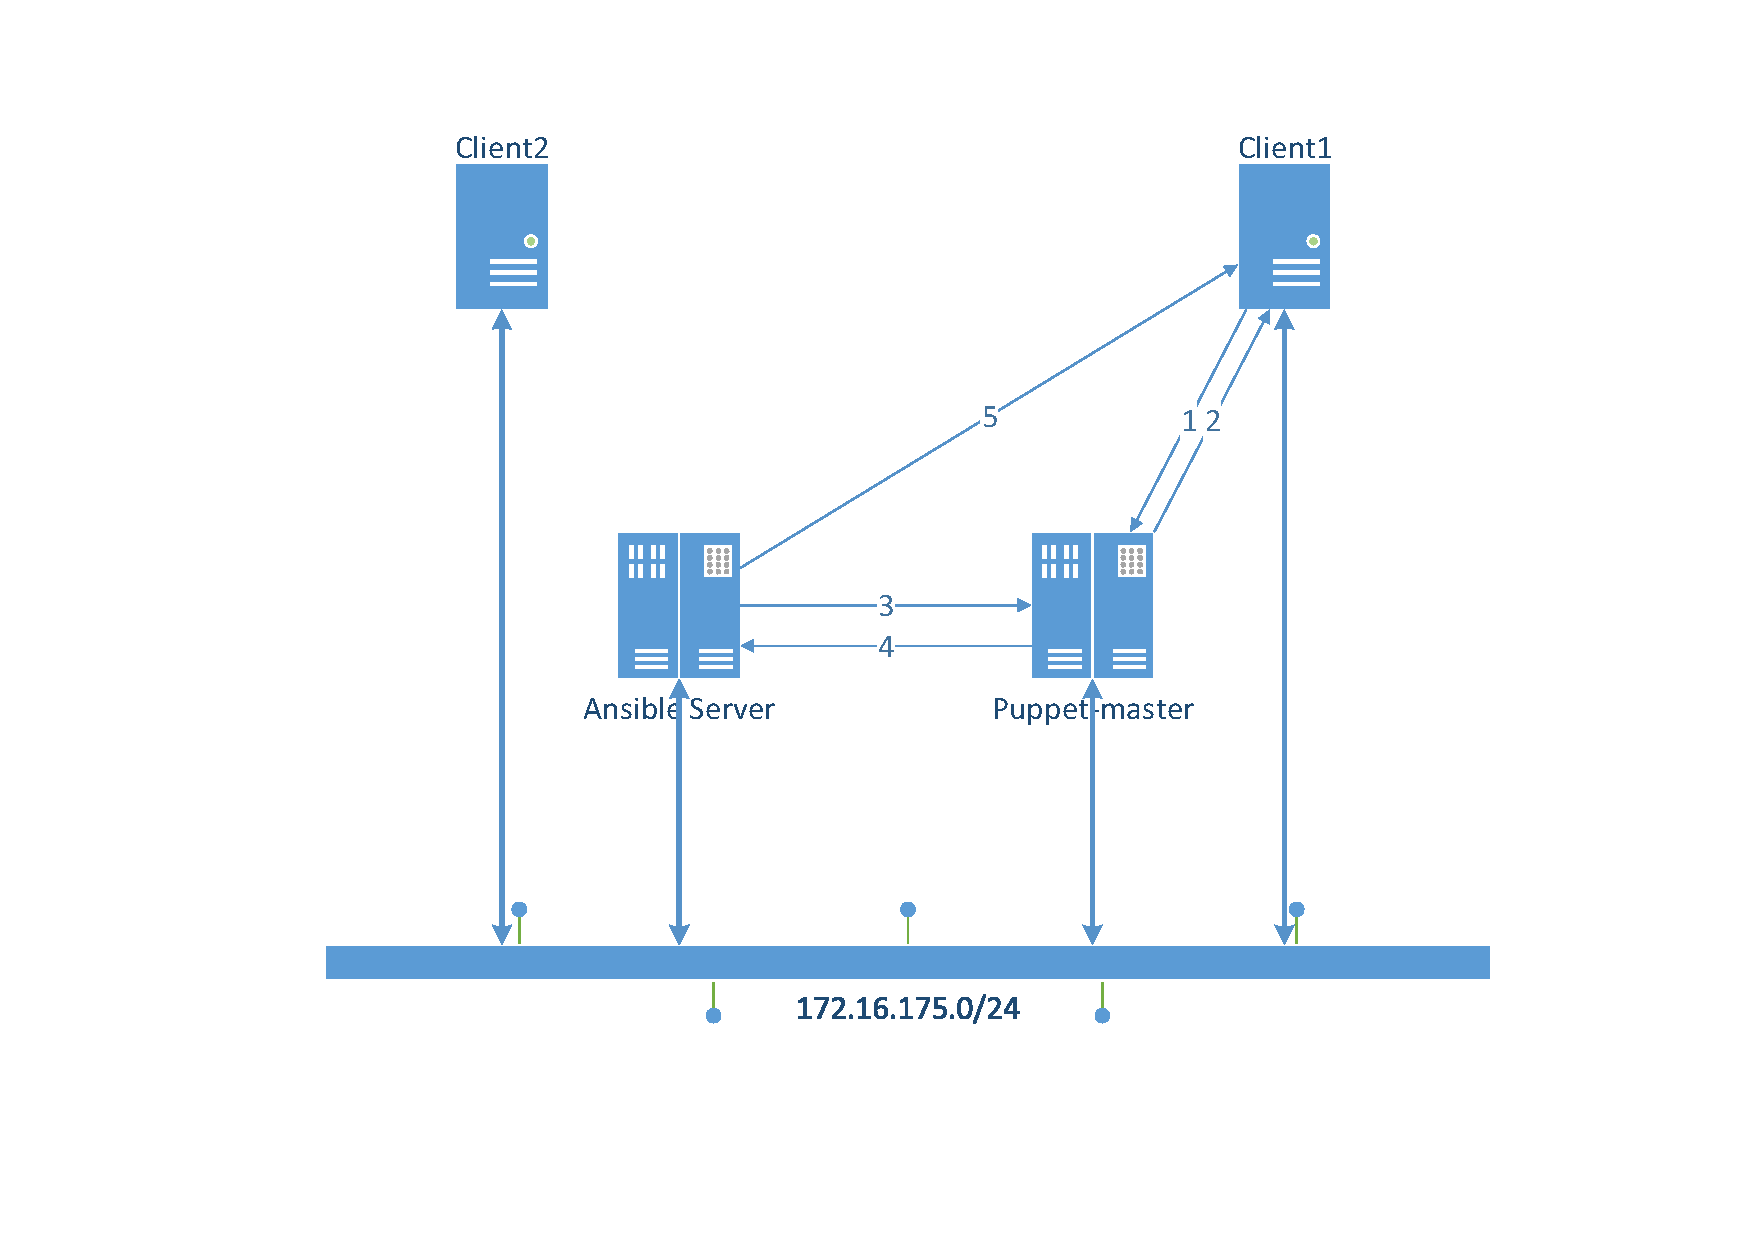
\includegraphics[scale=0.5]{img/PuppettoAnsible.pdf}     
        \caption{Migration from Puppet to Ansible.}
        \label{fig:situation1}
\end{figure}

\noindent
The migration scenario as presented in figure 2 shows a method for performing an in-place migration from Puppet to Ansible without affecting end users. The steps below describe how we envision a seamless migration in more detail:

\indent
\begin{itemize}
    \item[\bf Step 1] First, the Puppet clients need to be added to Ansible as a group. Ansible uses groups to target a subset of clients with a specific playbook. Adding the clients to the group is being done by leveraging Puppet. In order to enable Puppet to alter the Ansible configuration, a Puppet client needs to be installed on the Ansible server temporarily. This way the Puppet Master can send jobs to the Ansible server. Step one in figure 2 represents the installation of the Puppet agent on the Ansible server and the first check in of the Puppet agent to the Puppet Master.

    \item[\bf Step 2] Subsequently, the Ansible hosts file needs to be updated to contain the servers from the Puppet webservers group (Client1). Naturally, in a real world scenario, the hosts file step could be omitted and replaced with a reference to a DNS server.

    \item[\bf Step 3] After ensuring that the Ansible server can reach the clients, a Puppet job needs to be created for the Puppet clients which tells them to remove the Puppet agent from their system and allow SSH connections from the Ansible server. In step three the client checks in to the Puppet Master and receives the command set that tells the client to remove the Puppet agent.

	\item[\bf Step 4]
    In the fourth step, Client1 pulls the \texttt{puppet-enterprise-uninstaller} script from the Master. This uninstaller has to be automated and tasked to remove all files and packages related to the Puppet agent in order to guarantee a clean environment.

    % Welk playbook? Welke functie? Wat wordt er getest? Zeer onduidelijk.
    \item[\bf Step 5/6] When the Puppet webservers (Client1) are added to the Ansible system and the Puppet agent is removed from the clients the created playbook should be run. For this purpose, a Puppet job is created and steps five and six show the Puppet check in and retrieval of the command set. The new Ansible playbook is made and tested before changing the management system.
    
    \item[\bf Step 7] Finally, the Ansible server takes over the client by initiating an SSH connection and executing playbooks. This is the end of the client migration from Puppet to Ansible. As a last action the Puppet client can be removed from the Ansible server to fully decommission Puppet.
\end{itemize}

\noindent
One could argue that the full migration can be performed by leveraging Ansible exclusively, as this tool is able to uninstall the Puppet Agent as well by running the uninstaller script. However, we have opted to let Puppet deinstall the Puppet agent as this is a cleaner method per definition. allowing one to clean up certificate relationships between the Master and its clients. Additionally, by doing so, we can make sure that no errors occur during the deinstallation phase. If we would use Ansible exclusively, no feedback would be provided if the deinstallation would fail. Besides that, using Ansible for deinstallation would mean a hostile takeover of the system. 

\subsubsection{Migrating from Ansible to Puppet}\label{subsec:ansibletoPuppet}
Although this migration is most likely less frequently performed, it is still valuable in the sense of -for example- a fallback scenario. As with the previous migration scenario, before Ansible clients can be managed by the Puppet Master there are some prerequisites that need to be satisfied. The Ansible playbooks need to be reproduced in Puppet and the clients to be migrated need to be added to the correct Puppet groups. Otherwise they wont receive the correct packages. Additionally, when a client checks in at the Puppet Master for the first time, a certificate is exchanged. To prevent manual interaction this certificate should be accepted by default on the Puppet Master. In order for Puppet to accept all machine certificates an \texttt{autosign.conf} file can be created in the standard configuration directory \texttt{\$confdir}. The contents of this file function as a whitelist and are very restrictive by default. To accept all certificates, the only contents of this file should be a single wildcard '*'. This means that machines from all possible domains are accepted automatically. Naturally this poses security risks and would require sufficient segregation in a production environment.

\begin{figure}[!h]
        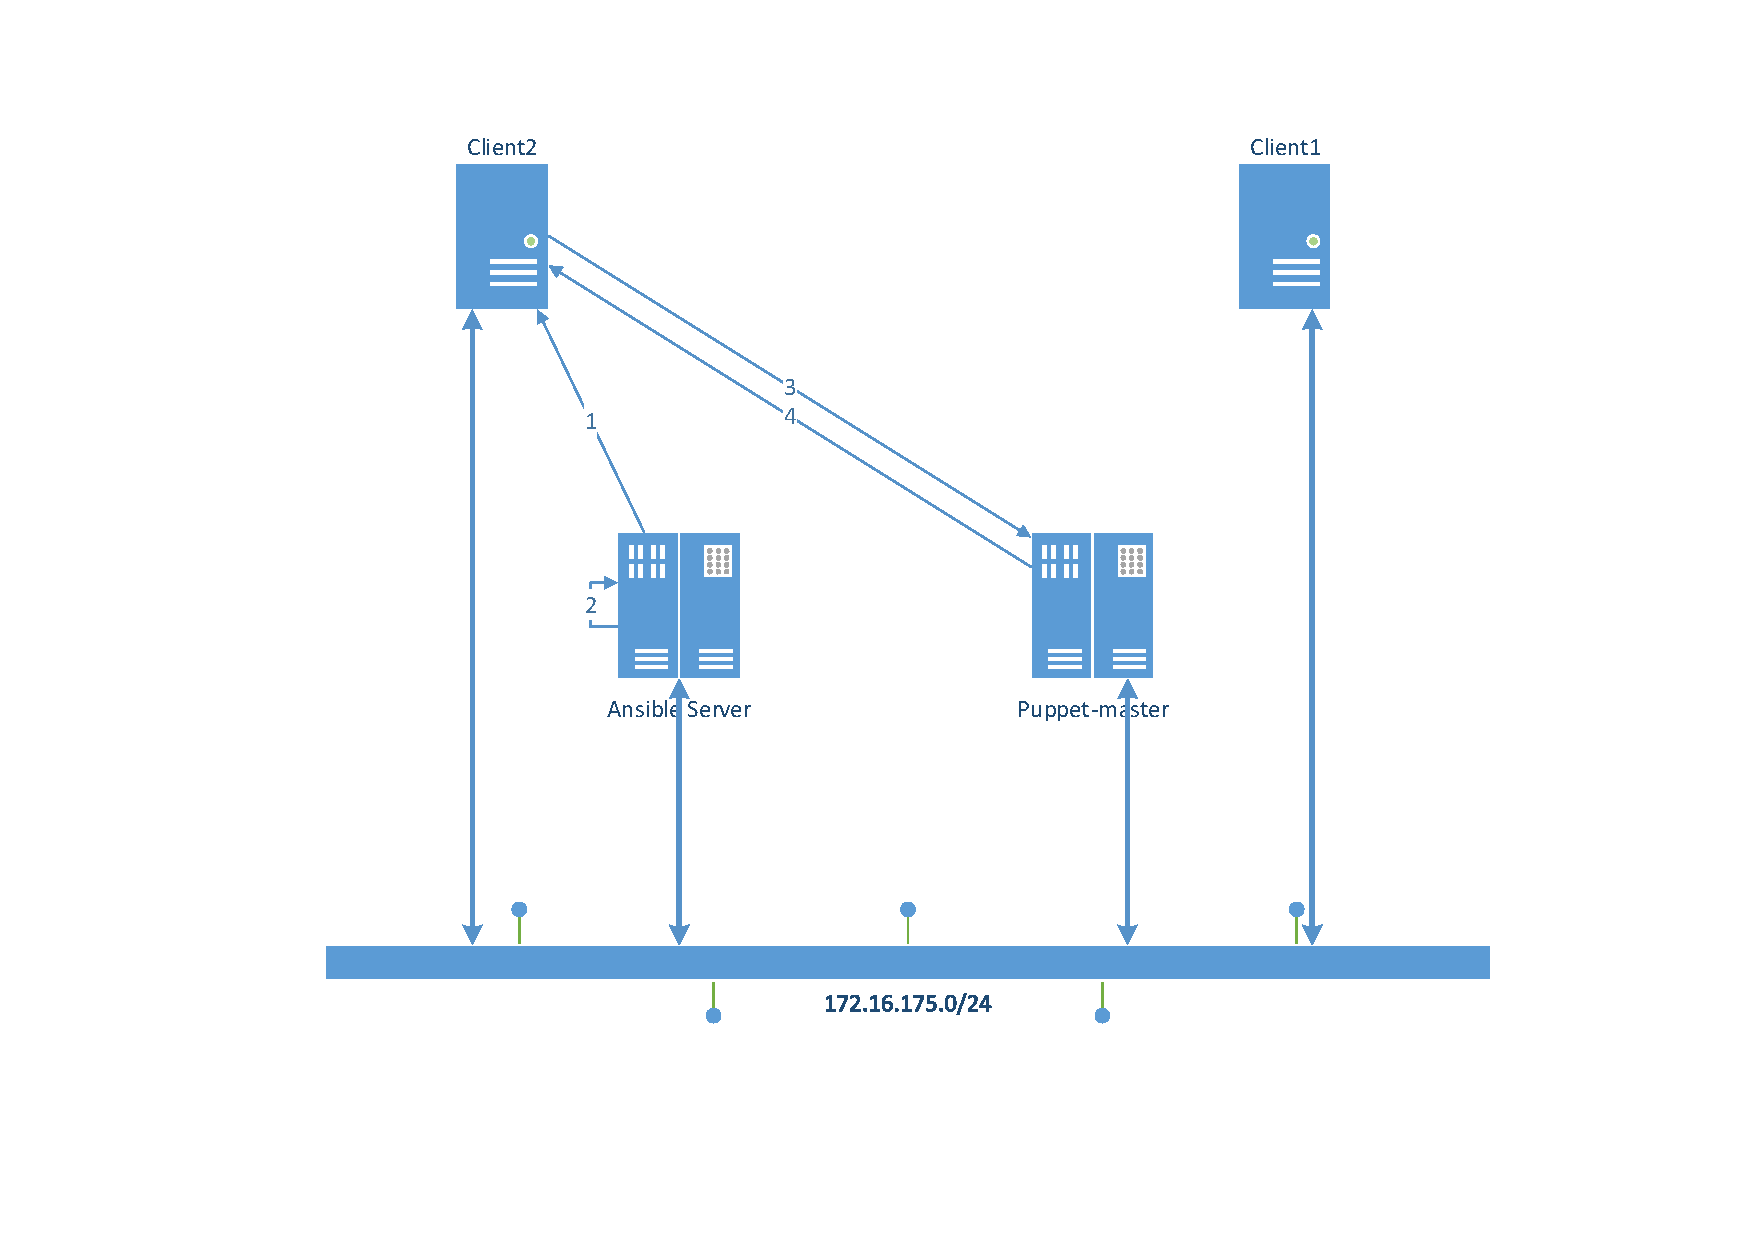
\includegraphics[scale=0.5]{img/AnsibletoPuppet.pdf}
        \caption{Migration from Ansible to Puppet.}
        \label{fig:situation2}
\end{figure}

The migration scenario as presented in figure 3 shows a method for performing an in-place migration from Ansible to Puppet without affecting end users. In figure \ref{fig:situation2} "Client2" is under control of the Ansible server. The steps below describe how we envision a seamless migration in more detail:

\indent
\begin{itemize}
    \item[\bf Step 1] Initially an SSH session from Ansible to the Puppet Master is initiated to add the client machines to the correct groups and prepare the \texttt{autosign.conf} file. 
    
    \item[\bf Step 2] Subsequently, the Ansible server sends the commands of this playbook to Client2. The full playbook is shown in section \ref{app:ansibleplaybook} of the appendixes and is discussed further in section \ref{sec:results}. An other way is to use the Puppet module within Ansible \cite{ansiblepuppet}. This uses the normal form of a playbook to install the Puppet client and the module to configure the Puppet client.     All machines managed by Ansible need to receive the Puppet agent in order to be managed by Puppet. This will be done by using an Ansible playbook. There are multiple ways to install the Puppet agent onto the client group represented in figure \ref{fig:situation2} as "Client2". In this methodology we opt to leverage a playbook with the command to install the Puppet agent using the bash installer provided by the Puppet Master.

    \item[\bf Step 3] When the playbook is sent to the Ansible clients the clients need to be removed from the Ansible hosts file. Therefore the end of the playbook should contain a change into the local Ansible hosts file show in the picture as step three.

    \item[\bf Step 4] Step four shows the first check in from Client2 into Puppet to get the correct version and check in for available jobs.

    \item[\bf Step 5] Lastly, step five represents the Puppet jobs to be transferred to the client. From this moment onwards the system is managed by Puppet instead of Ansible.

\end{itemize}

To perform the migration in an automated fashion all the described steps will be put into a Playbook and a Puppet module.

\subsubsection{Automation factor}\label{subsec:expectations}
% Onduidelijk. Wat is nu eigenlijk echt het probleem? En waarom is dit een verwachting?
For the migration between systems, especially when moving away from a pull based system like Puppet the system needs to be expanded first as explained in the first part of this chapter. The Puppet agent needs to be installed on the Ansible server to make sure the client is added to the host list and the playbook is run in the appropriate time. But there we run into the big disadvantage of Puppet, when using puppet and there are multiple different jobs within one task. You cannot tell what jobs are executed first without special commands. So in order to make this work different jobs need to be prepared and some relations could be created within Puppet. If step one succeeds, proceed to step two, and so on. If step one fail, make a notification and stop the process.  

\subsection{Mgmt experiments}
The second test scenario will be used to perform a deployment of an Apache webserver on a single node (Ubuntu 14.04 LTS) using \texttt{mgmt}. Whilst doing so, the capabilities of \texttt{mgmt} to perform parallel execution of tasks will be examined. The scenario in figure \ref{fig:parallelexec} exhibits parallel execution of processes within \texttt{mgmt} by presenting two disjoint graphs in which the left graph installs the \texttt{apache2} package and generates an index and a style file in parallel. The graph on the right sequentially runs sleep commands in parallel with the \texttt{apache2} installation. Naturally, a real-world deployment would include meaningful commands in this parallel graph, such as the installation of a database for example.  

\begin{figure}[!ht]
  \begin{center}
          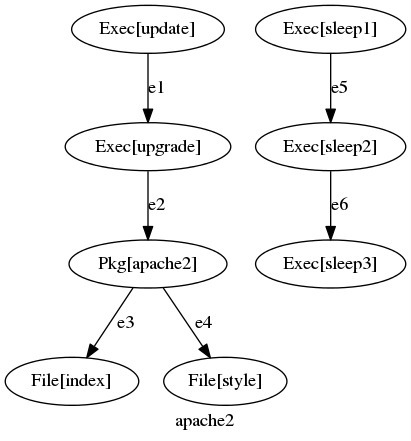
\includegraphics[scale=0.44]{img/graph.jpeg}
          \caption{Parallel execution proof of concept with Apache2 installation}
          \label{fig:parallelexec}
  \end{center}
\end{figure}

Subsequently the (re)convergence speed of the tool will be tested by changing the contents of a file and by removing the \texttt{apache2} software package -and its dependencies- from the system. By performing this experiment we aim to illustrate the advantages which \texttt{mgmt} poses over traditional configuration management tools. Our main aim is to visualize the speed increase in state reconvergence when a deviation is created in the desired state. By removing the Apache web server we can measure how long downtime would approximately occur in a small scale environment.

\noindent
It should be noted that we do not examine the potential scalability of \texttt{mgmt} due to resource constraints. Additionally, there are no official numbers available to compare the scalability of the CMS tested in this report. We discuss the scalability of a distributed configuration management system and the implications of our test scenario further in section \ref{sec:discussion}.  
